\documentclass[utopia]{nmd/article}
\pdfoutput=1
\usepackage{amssymb,epic,eepic,epsfig}%,amsbsy,amsmath,bbold}

\def\BC{\mathbb C}
\def\Li{\mathrm{Li}}
\def\Stirling#1#2{\left\{\!\begin{array}{c}#1\\#2\!\end{array}\right\}}

\title{Verified computations\\ \mbox{} \hspace{5cm}  of the polylogarithm}

\author{Matthias Goerner}
\email{enischte@gmail.com}
\urladdr{http://unhyperbolic.org/}

\begin{document}

\begin{abstract}
We review existing formulas to show how to compute a complex interval arithmetic polylogarithm for integral orders and related functions giving the (complex) volume of hyperbolic 3-manifolds.
\end{abstract}

\maketitle

\section{Introduction}

The polylogarithm is defined as the analytic continuation of the series

\begin{equation} \label{eqn:def}
\Li_{n}(z) = \sum_{k=1}^{\infty} \frac{z^k}{k^n}
\end{equation}
It is a generalization of the logarithm with $\Li_1(z) = -\ln(1-z)$. $\Li_2$ is known as the dilogarithm - the only function with a ``sense of humor'' according to Zagier's excellent survey article \cite{zagier:theDilogarithmFunction}.\\
We will review the necessary identities and series and give error estimates to implement a complex interval version of the polylogarithm for integral orders.\\
The input to such a polylogarithm is the integeral order $n$ and a complex interval which is a rectangle $K=\big[\underbar{a},\overline{a}\big]+\big[\underbar{b},\overline{b}\big]i\subset\mathbb{C}$
in the complex plane where $\underbar{a}, \overline{a}, \underbar{b},$ and $\overline{b}$ are real numbers exactly representable by floating point numbers. A correct implementation must return another complex interval $L$ such that for every $z\in K$, we have $\Li_n(z)\in L$ --- at least as long as $K$ does not intersect the branch cut at $[1,\infty)$, see Chapter~\ref{}. The returned interval $L$ should be reasonably small but does not need to be the smallest interval possible with this property.\\
We use methods similar to the ones in the Pari \cite{pari} library, but deploy interval arithmetic. A technical report similar to this one is \cite{wood92}.\\
Before describing these methods, we review related functions that can be applied to compute volumes of hyperbolic 3-manifolds.

\section{Semantics of complex interval arithmetics}

\subsection{Differences to MPFI}

Let $f:\mathbb{R}^n\to \mathbb{R}$ be a function. We say that an interval implementation of $f$ is correct if it returns an interval $J$ given some real input intervals $I_1, \dots I_n$ such that $f(x_1,\dots, x_n)\in J$ whenever $x_j\in I_j$ for $j=1,\dots, k$. Note that this does not require the interval implementation to
\begin{enumerate}
\item be deterministic, i.e., two calls of the same functions given the same inputs might return two different intervals \label{weakest}
\item preserve inclusions, i.e., if $I'_j\subset I_j$ for $j=1,\dots, k$, then $J'\subset J$ where $J'$ is returned when giving the $I'_j$ as inputs. \label{inclusion}
\item return the smallest possible interval that has as endpoints floating-point numbers of the given precision. \label{strongest}
\end{enumerate}
The MPFI library implements real interval arithmetics and most (if not all) of its function satisfy the strongest condition (\ref{strongest}). Given how hard it is to achieve the analogous conditions for complex functions and intervals, a library for complex interval arithmetic might choose to implement functions in such a way that the returned intervals are still correct but only fulfill condition (\ref{weakest}).

\subsection{Interpretations of multi-valued functions} The MPFI library implements the $\arg(y,x)$ function which returns the signed angle of the $x$ axis and the line segment from the origin to the point $(x,y)$. If we give it as input intervals $[-1,-1]$ for $x$ and $[-0.0625,0.0625]$ for $y$, it returns $[\underline{-\pi},\overline{\pi}].$\\
In a complex analysis setting, it is more natural to think of a function such as $\log$ (whose imaginary part is given by $\arg$) as being multi-valued. The $\log$ function is related to the $\exp$ function which is a covering map $\C\to\C\setminus 0$. A complex interval implementation can be thought of as returning a particular lift of a given complex interval in $\C\setminus 0$ to $\C$. This requires a choice and it is canonical to pick a lift that agrees with the logarithm's principal value if the complex interval avoids the branch cut at $(-\infty, 0)$.\\
Some examples of the results returned by the complex interval logarithm will make this more clear (note that (\ref{inclusion}) is not satisfied):\\
\begin{tabular}{ll|llllll}
&\multicolumn{1}{c|}{$z$} & \multicolumn{1}{c}{$\log(z)$}\\ \hline
&[-1,-1]+[\phantom{-}0.0625, \phantom{-}0.0625]i & [0.00194, 0.00196] + [\phantom{-}3.0791, \phantom{-}3.080\phantom{0}]i\\
&[-1,-1]+[\phantom{-}0\phantom{.0625}, \phantom{-}0.0625]i & [0\phantom{.00194}, 0.00196] + [\phantom{-}3.0791, \phantom{-}3.1416]i\\
&[-1,-1]+[-0.0625, \phantom{-}0.0625]i & [0\phantom{.00194}, 0.00196] + [\phantom{-}3.0791, \phantom{-}3.2041]i\\
&[-1,-1]+[-0.0625, \phantom{-}0\phantom{.0625}]i & [0\phantom{.00194}, 0.00196] + [\phantom{-}3.1415, \phantom{-}3.2041]i\\
&[-1,-1]+[-0.0625, -0.0625]i & [0.00194, 0.00196] + [-3.080\phantom{0}, -3.0791]i\\
\end{tabular} \medskip \\
This is justified by the fact that clients calling $\log$ or $\sqrt{z}$ (which can be implemented as $\exp(\log(z)/2)$) often care about the result only up to multiplies of $2\pi i$, respectively, sign.\\ 
Evaluating $\log$ on a complex interval containing $0$ is not allowed which can be signaled by returning NaN (Not a Number).\\
Similarly, the polylogarithm has a singularity at 1 and the branch cut of polylogarithm is typically chosen to be $(1,\infty)$. For consistency, evaluating the polylogarithm on a complex interval containing $0$ should not be allowed either, even though the singularity is such that the principal value of polylogarithm converges as $z\to 1$.

\subsection{A subtle pitfall} Let $z$ be some complex quantity such as the cross ratio of an ideal tetrahedron. While an algorithm using the complex interval library typically does not care which of the two values for $\sqrt{z}$ the library chooses, it might still require that every occurrence of $\sqrt{z}$ returns the same choice.\\


While algorithms implemented by a client of a complex interval library typically do not care about the choice of $\sqrt{z}$, they still might require that whenver 

Mathematically, the following holds
$$c=\lambda_0 \lambda'_0 = \lambda_1 \lambda'_1$$
One choice $\sqrt{c}$. Interval implementation: $\sqrt{\lambda_0 \lambda'_0}$ and $\sqrt{ \lambda_1 \lambda'_1}$.

\section{Related functions}

The dilogarithm
$$\Li_2(z) = -\int_0^z \frac{\log(1-t)}{t}dt$$
can be used to compute the Lobachevsky function
$$L(\theta)=-\int_0^\theta \log |2\sin(t)| dt = \frac{1}{2} \mathrm{Im}\left(\Li_2\left(e^{2i\theta}\right)\right),$$
the Bloch-Wigner function
$$D(z)=\mathrm{Im}\left(\Li_2(z)\right) + \arg(1-z)\log|z|,$$
and Roger's dilogarithm
$$\mathcal{R}(z)=\Li_2(z)+\frac{1}{2}\log(z)\log(1-z)$$
which Neumann \cite{Neumann} uses to define
$$R(z;p,q)=\mathcal{R}(z)+\frac{\pi i}{2}\left(p\log(1-z)+q\log(z)\right)-\frac{\pi^2}{6}.$$
The Lobachevsky function and Bloch-Wigner function can be used to compute the volume of a hyperbolic ideal 3-simplex from its three dihedral angles, respectively, its cross-ratio as explained by Milnor \cite{Milnor}. Neumann's $R(z;p,q)$ relates to the extended Bloch group and can be used to compute the complex volume of a hyperbolic 3-manifold.



\section{General strategy}

If $n\leq 0$, $\Li_n$ is actually a rational function which we treat separately in Section~\ref{}. For $n=1$, we have $\Li_1=-\ln(1-z)$, so we are only concerned about orders greater than 1 here.\\
If $|z|<1$, we can use the defining series \eqref{eqn:def} and, if $|z|>1$, Jonqui\`e{}re's inversion formula 
 \cite{jonquiere89}
 \begin{equation} \label{eqn:inversion}
\Li_n(z) =  -\left( \frac{(2\pi i)^n}{n!} B_n\left(\frac{\ln(z)}{2\pi i}\right) + (-1)^n \Li_n(1/z) \right)
\end{equation}
reduces the problem to the case $|z|<1$ where
$$B_n(x)=\sum_{k=0}^n {n \choose k} b_{n-k} x^k = - \sum_{k=0}^n \frac{n (n-1) \dots (n-k)}{k!} \zeta(k-n+1) x^k$$
is the Bernoulli polynomial and $b_i$ are the Bernoulli numbers.\\
The resulting series converges arbitrarily slow though when $|z|$ is close to 1. In this case, we can use the following series for $z=e^\mu$ with $|\mu|<2\pi$%\cite[\S 9]{wood92}, \cite[\S 9.554]{gradshteynRyzhik80}:

\begin{equation} \label{eqn:series1}
\Li_n (e^\mu) = \frac{\mu^{n-1}}{(n-1)!} \left[\sum_{h=1}^{n-1} \frac{1}{h} - \ln(-\mu)\right] + 
\sum_{k=0,k\not=n-1}^\infty \frac{\zeta(n-k)}{k!} \mu^k.
\end{equation}
Section~\ref{} discusses the interval implementation of these series giving error bounds. This also enables us to analyze the convergence speed of these series in Section~\ref{} which tells us which series to pick for a given $z$ to make the computation of the polylogarithm faster.\\
If the given interval for $z$ is so large that none of $|z|<1$, $|z|>1$, or $|\mu|<2\pi$ hold, an interval implementation can simply give $(-\infty, \infty) + (-\infty, \infty)i$ as result.

\begin{remark}
None of the series performs well (gaining less than 2 bits precision per term) when $z$ is close to -0.3 (see Figure~\ref{fig:convergenceSpeed}) and there is a potential optimization by using the duplication formula \cite{clunie54, schroedinger52}
$$\Li_n(z) = 2^{1-n} \Li_n(z^2) - \Li_n(-z).$$
\end{remark}



\section{Error bounds on the series}

\subsection{Error bounds}

Let $E[r]=[-r,r]+[-r,r] i$. For the series about 0 from Equation~\ref{eqn:def}, we have $|t_k+1| < r|t_k|$ with $r=|z|$ for two subsequent terms. This means that the absolute value of the sum of the terms after $t_u$ is bounded by a geometric series with common ratio $r$ and we obtain
\begin{equation} \label{eqn:defSeriesInterval}
\Li_n(z)\in \sum_{k=1}^u t_k + E\left[F\cdot \left| t_u\right|\right]\mbox{ where } t_k = \frac{z^k}{k^n} \mbox{ and } F=\frac{r}{1-r} \mbox{ with } r=|z|.
\end{equation}
Similarly, we have for the series about 1 from Equation~\ref{eqn:series1}
\begin{equation} \label{eqn:series1interval}
\Li_n(e^\mu)\in \frac{\mu^{n-1}}{(n-1)!} \left[\sum_{k=1}^{n-1}\frac{1}{k} - \ln(-\mu)\right] + \sum_{k=0}^{n-2} t_k + t_n + \sum_{k=n+1}^u t_k + E\left[F\cdot \left|t_u\right|\right]
\end{equation}
$$ \mbox{ where } t_k=\frac{\zeta(n-k)}{k!} \mu^k \mbox{ and } F=\frac{r}{1-r} \mbox{ with } r=|\mu/(2\pi)|^2$$
when $u$ and $n$ have the opposite parity and $u\geq n+1$. It follows from Riemann's functional equation
\begin{equation}\label{eqn:riemann}
\zeta(s) = 2^s \pi^{s-1} \sin\left(\frac{\pi s}{2}\right) \Gamma(1-s)\zeta(1-s),
\end{equation}
that every other term $t_{n+2}, t_{n+4}, ...$ in the last sum is zero and that the non-trivial terms in the last sum are given
$$t_k = 2(2\pi)^{n-1} (-1)^{\left(\frac{k-n+1}{2}\right)} \frac{\zeta(k-n+1)}{k(k+1)\cdots(k-n+1)} \left(\frac{\mu}{2\pi}\right)^k \mbox { for } k=n+1,n+3, \dots~ .$$
Since the Riemann $\zeta$-function is descreasing on $(1, \infty)$, we also see that $|t_{k+2}| < r |t_k|$ where $r=|\mu/(2\pi)|^2$ and thus obtain the above error bound $F\cdot |t_u|$.

\subsection{Interval arithmetic implementations} To be able to use \eqref{eqn:defSeriesInterval} or \eqref{eqn:series1interval}, we first need to use interval arithmetics to verify that $|z|<1$, respectively, $|\log(z)| < 2\pi$.\\
For all the operations on the right hand side of these two formulas, 
we apply the corresponding interval versions except for the term $E[F\cdot |t_u|]$ which we need to replace by $E[\overline{F\cdot |t_u|}]$ where $\overline{F\cdot |t_u|}$ is obtained by applying interval arithmetic to compute an interval for $F\cdot |t_u|$ and picking the right endpoint of that interval (since we don't use the left endpoint of the interval, we can save some work by computing only $\overline{F\cdot |t_u|}$ by proper rounding).\\
More technical notes: An interval implementation could evaluate the right hand side of \eqref{eqn:defSeriesInterval} or \eqref{eqn:series1interval} for larger and larger $u$ until the resulting complex interval is not descreasing in size anymore. We also get tighter complex intervals as result by doing intermediate computations in slightly higher precision. Subsequent evaluations of polylogarithms by \eqref{eqn:series1interval} can be sped up significantly by caching the values of the Riemann $\zeta$-function.

\section{Convergence speed}
We gain about $-\log_2(|z|)$ bits of precision per term when using Equation~\ref{eqn:defSeriesInterval} and $-\log_2(1/|z|)$ when combining that equation with the inversion formula. Similarly, we gain about $-\log_2((|\log(z)|/2\pi)^2)$ bits of precision for each non-trivial term when using Equation~\ref{eqn:series1interval}.\\
Thus, we prefer using Equation~\ref{eqn:series1interval} when
\begin{equation} \label{eqn:whichSeries}
(|\log(z)| / 2\pi)^2 < \min(|z|, 1/|z|).
\end{equation}
Figure~\ref{fig:convergenceSpeed} shows the convergence speed of series \eqref{eqn:series1} and the region where this series converges faster than \eqref{eqn:def}. The convergence is slowest near -0.3 where both series gain only about 1.7 bits per term.\\
When we test for \eqref{eqn:whichSeries} in code, we do not need to use interval arithmetic or higher precision to verify it since the wrong choice will still be correct, just slower to compute (as long as $z$ in the domain where the chosen series still converges).\\

\begin{figure}
\begin{center}
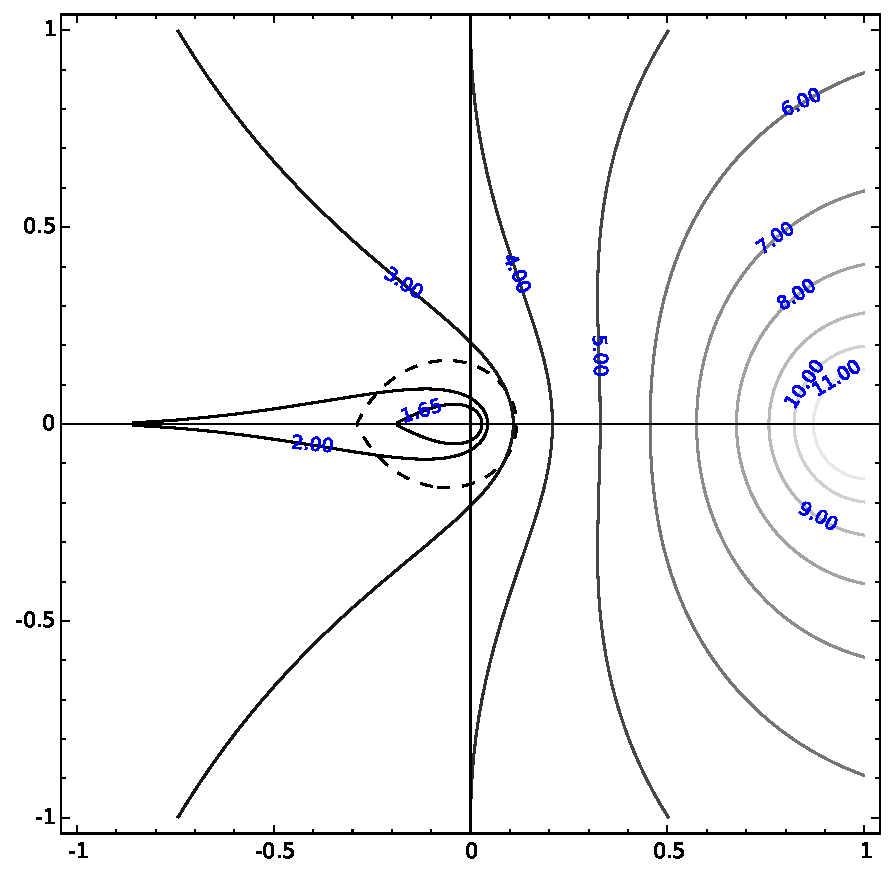
\includegraphics[height=9cm]{implementation_polylog_speed.pdf}
\end{center}
\caption{Bits precision per non-trivial term $t_k$ in \eqref{eqn:series1}. The dashed line encloses the region where series \eqref{eqn:def} converges faster than \eqref{eqn:series1}. The picture is invariant under inversion $z\mapsto 1/z$.}
\label{fig:convergenceSpeed}
\end{figure}




\section{Non-positive integral orders}

For $n\geq 0$, the polylogarithm $\Li_{-n}$ is obtained by applying $(n+1)$ times the operator $z \frac{\partial \_}{\partial z}$ to $\Li_1(z)=-\ln(1-z)$. It is thus a rational function given by %\cite[\S 6]{wood92}
$$\Li_{-n}(z) = \sum_{k=0}^n k!~ \Stirling{n+1}{k+1} ~ \left(\frac{z}{1-z}\right)^{k+1}$$
where $\Stirling{n}{k}$ are the Stirling numbers of second kind given explicitly by
\begin{equation} \label{eqn:stirlingExplicit}
\Stirling{n}{k} = \frac{1}{k!} \sum_{j=0}^k (-1)^{k-j} {k \choose j} j^n
\end{equation}
or recursively by
$$\Stirling{n+1}{0} = 0,\quad \Stirling{n+1}{k} = k \Stirling{n}{k} + \Stirling{n}{k-1}\quad\mbox{for}\quad k > 0$$
and the initial conditions $$\Stirling{0}{0}=1,\quad \Stirling{0}{k}\quad\mbox{for}\quad k > 0.$$
Note that the recursive definition is easy enough for a numerical implementation and also preferable over 
\eqref{eqn:stirlingExplicit} since it avoids the alternating sum that could potentially accumulate larger errors.

\section{Bernoulli numbers and Riemann $\zeta$-function}

\subsection{Bernoulli numbers}
The Bernoulli numbers can be defined recursively:
\begin{equation} \label{eqn:bernoulliDef}
b_m = 1 - \sum_{k=0}^{m-1} {m\choose k} \frac{b_k}{m-k+1}\quad\mbox{for}\quad m\geq 0.
\end{equation}
This also allows to compute the Riemann $\zeta$-function for odd negative integers and even positive integers
$$\frac{b_{2n}}{2n} = -\zeta(1-2n) = (-1)^{n+1} \frac{2(2n-1)!}{(2\pi)^{2n}} \zeta(2n)\quad\mbox{for}\quad n\geq 1.$$
The latter equation directly follows from Riemann's functional equation \ref{eqn:riemann} which also implies that $\zeta$ is zero at the even negative integers. Furthermore, we have $\zeta(0)=-1/2$.\\
For our purposes, we can use \eqref{eqn:bernoulliDef} to compute the Bernoulli numbers. Pari employs a different algorithm, but it has different goals: compute a Bernoulli number $b_m$ for much higher $m$ with high enough precision to obtain a rational representation of $b_m$ and without computing all the pervious Bernoulli numbers. Pari's algorithm computes $\zeta$ using the Euler product which actually converges quickly if $m$ is large and uses that von Staudt and Clausen give an expression for the numerator of $b_m$, see \cite{mcgown:bernproj,stein:bernproj}.

\subsection{Riemann $\zeta$-function at positive odd integers}
To compute higher polylogarithms, we still need a way to compute the values of $\zeta$ at the odd positive integers. Ramanujan gave a formula for these:
\begin{multline}
(-\alpha)^{-n}\left[\frac{\zeta(2n+1)}{2} + \sum_{k=1}^\infty \frac{k^{-2n-1}}{e^{2\alpha k}-1}\right]-
\beta^{-n}\left[\frac{\zeta(2n+1)}{2} + \sum_{k=1}^\infty \frac{k^{-2n-1}}{e^{2\beta k}-1}\right]=\\
2^{2n} \sum_{k=0}^{n+1} (-1)^k \frac{b_{2k}}{(2k)!} \frac{b_{2n+2-2k}}{(2n+2-2k)!} \alpha^k \beta^{n+1-k} \label{eqn:ramanujan}
\end{multline}
where $n$ is a positive integer and $\alpha\beta=\pi^2, \alpha, \beta > 0$, proven, for example, by Berndt \cite{berndt:ramanujan}. If $(-\alpha)^{-n}-\beta^{-n}\neq 0$, we can solve for and quickly compute $\zeta(2n+1)$. In particular, for $n$ odd and $\alpha=\beta=\pi$, we obtain
$$\zeta(4m-1) =  - \frac{1}{2}(2\pi)^{4m-1}\sum_{k=0}^{2m} (-1)^k \frac{b_{2k}}{(2k)!} \frac{b_{4m-2k}}{(4m-2k)!} -2 \sum_{k=1}^\infty \frac{1}{k^{4m-1}\left(e^{2\pi k} - 1\right)}.$$
for $m\geq 1$ which converges quickly ($e^{2\pi}=535.49...$). For $n$ even, we can take the derivative of equation \eqref{eqn:ramanujan} and again set $\alpha=\beta=\pi$ to obtain
\begin{multline}
\zeta(4m+1) =\\ \frac{(2\pi)^{4m+1}}{2m} \sum_{k=0}^m (-1)^k (2m+1-2k) \frac{b_{2k}}{(2k)!} \frac{b_{4m+2-2k}}{(4m+2-2k)!} - 2 \sum_{k=1}^\infty \frac{e^{2\pi k} (1 + \pi k / m) - 1}{k^{4m+1}(e^{2\pi k}-1)^2}.
\end{multline}
These equations are also used by pari and, according to Cohen \cite{cohen:hardyLittlewood}, can also be proved ``by computing the period functions associated to the Eisenstein series of weight $4m+2$ on $\mathrm{PSL}(2,\mathbb{Z})$''.%\\
%Other equations for $\zeta$ at positive odd integers are given by Vepstas.





\section{STUFF}

\begin{verbatim}
C=contour_plot(
    lambda x,y:-log(abs(log(x+y*I))/6.283)/0.3465735+log(abs(x+y*I))/0.693147,
    (-1,1),(-1,1),
    axes=True,contours=[0],linestyles='dashed',
    fill=False,plot_points=300)
C2=contour_plot(
    lambda x,y:-log(abs(log(x+y*I))/6.283)/0.3465735,
    (-1,1),(-1,1),
    axes=True,contours=[1.65,2,3,4,5,6,7,8,9,10,11],
    fill=False,plot_points=300, labels=True)
C3=C+C2
\end{verbatim}

%\url{http://arxiv.org/abs/math/0609775}



\bibliographystyle{nmd/math}
\bibliography{implementation}



\end{document}
